\section{Strutture dati spaziali}
\label{sec:strutture_dati_spaziali}

Molti algoritmi di elaborazione geometrica richiedono, come operazione di base, di rispondere in modo efficiente a interrogazioni di prossimità tra punti: dato un punto $p$, trovare tutti i punti $p'$ che distano da esso meno di una soglia $r$ fissata. Questo problema è noto in letteratura come \emph{fixed-radius near-neighbor problem} e può essere formalizzato come segue:
\[
\text{dato } p, \text{ trovare } \{p' : d(p, p') < r\}
\]

dove $d$ è la distanza euclidea. Un approccio diretto (\emph{naive}) consiste nel confrontare ogni punto con tutti gli altri, con una complessità $O(N)$ per ogni singola interrogazione e quindi $O(N^2)$ per elaborare un intero insieme di $N$ punti: un costo che diventa rapidamente insostenibile al crescere della dimensione dell'insieme. Per questo motivo, quando il numero di interrogazioni è elevato, è preferibile appoggiarsi a una struttura dati pensata per organizzare i punti nello spazio e restringere la ricerca ai soli candidati plausibili.

\subsection{Approcci alla ricerca di prossimità}

Le strutture dati più diffuse per questo tipo di problema si dividono in due grandi famiglie. La prima è quella delle strutture gerarchiche di partizionamento dello spazio, come il \emph{K-D Tree} o il \emph{quadtree}, che suddividono ricorsivamente lo spazio in regioni via via più piccole organizzate in un albero. Queste strutture garantiscono interrogazioni di vicinanza in tempo $O(\log N)$.

La seconda famiglia è quella delle strutture basate su una griglia regolare, tra cui l'\emph{hash spaziale} (\emph{spatial hash}). A differenza delle strutture ad albero, un hash spaziale non organizza i punti in una gerarchia, ma li distribuisce in \emph{bucket} (celle) di una griglia uniforme, usando le coordinate del punto stesso come chiave di hashing. Questo approccio è più semplice da implementare, supporta inserimenti e rimozioni in tempo pressoché costante, ed è particolarmente indicato quando il raggio di ricerca $r$ è noto a priori \cite{autoware_spatial_hash}.

\subsection{L'hash spaziale}
\label{subsec:hash_spaziale_teoria}

Il funzionamento di un hash spaziale si basa su un'idea semplice: lo spazio 2D viene suddiviso in una griglia regolare, in cui ogni cella ha una dimensione fissa. A ciascun punto viene associata esattamente una cella, calcolata a partire dalle sue coordinate. L'insieme dei punti che ricadono nella stessa cella viene poi memorizzato in una struttura hash (ad esempio una \texttt{unordered\_map} o una \texttt{unordered\_multimap}), la cui chiave è la coppia di indici che identifica la cella.

La proprietà che rende questa struttura efficiente per le interrogazioni di prossimità è la seguente: se la dimensione della cella è scelta pari al raggio di ricerca $r$, due punti che distano meno di $r$ si trovano necessariamente nella stessa cella oppure in una delle celle immediatamente adiacenti. Questo significa che, per rispondere a un'interrogazione centrata in un punto $p$, non è necessario esaminare l'intero insieme di punti, ma è sufficiente calcolare la cella di appartenenza di $p$ ed esaminare unicamente le celle vicine (una griglia $3 \times 3$), effettuando un confronto esplicito di distanza solo con i punti che vi ricadono.

\begin{figure}[htp]
	\centering
	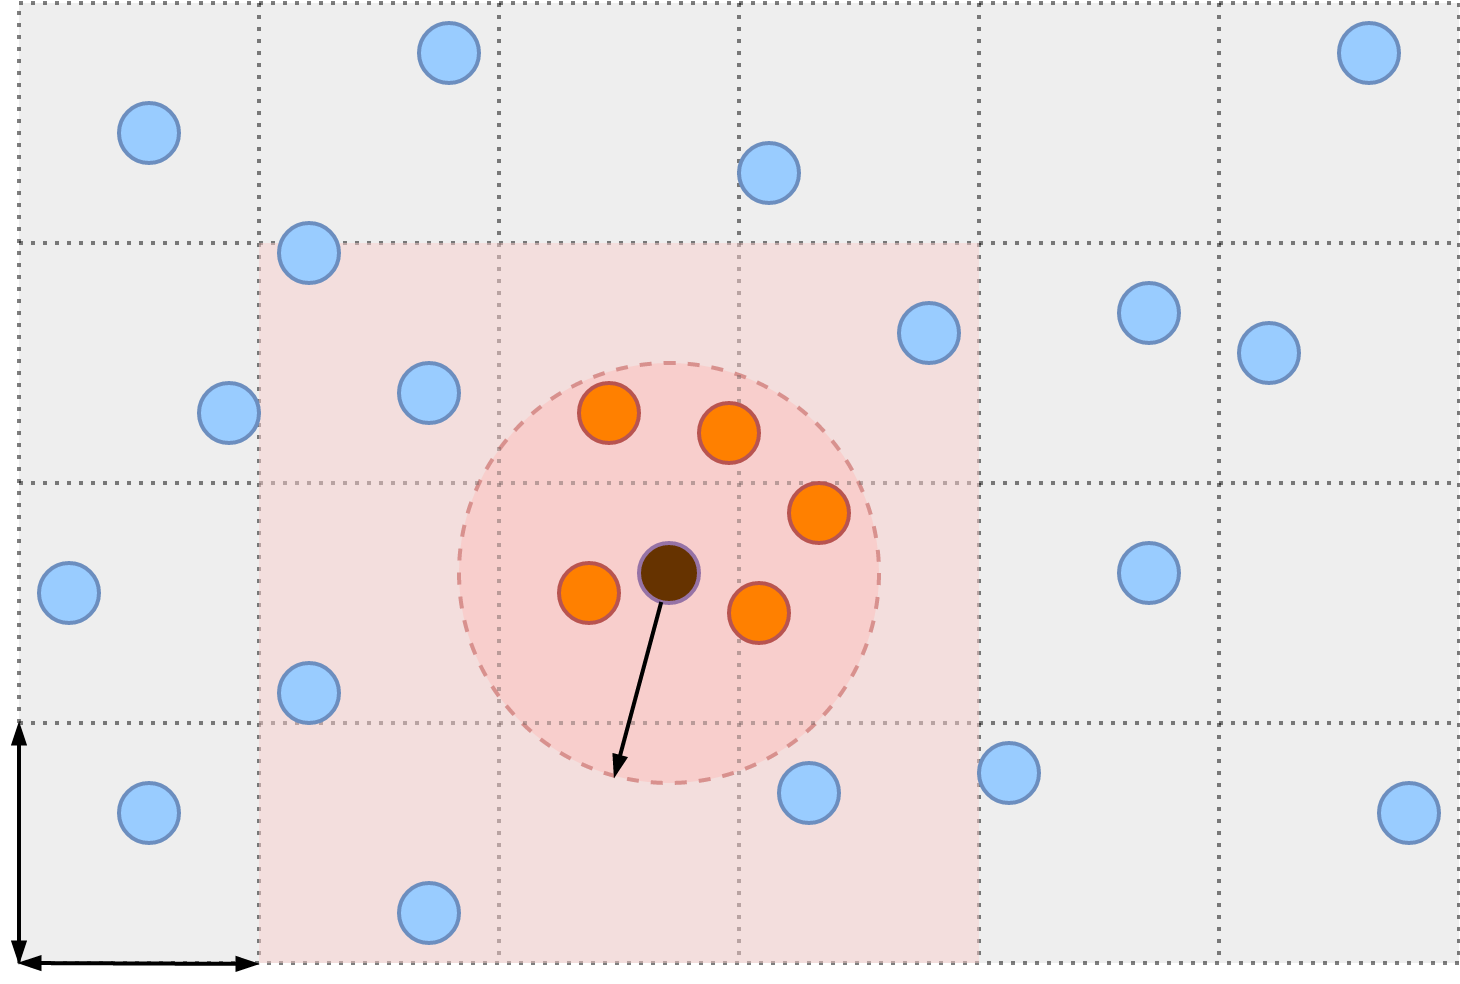
\includegraphics[width=0.5\textwidth]{figures/2_background_teorico/cell_list.png}
	\label{fig:cell_list}
\end{figure}

\subsection{Complessità e scelta della dimensione della cella}

L'inserimento di un nuovo punto ha complessità $O(1)$. Analogamente, un'interrogazione di prossimità ha complessità $O(k)$, dove $k$ è il numero medio di punti contenuti nelle celle esaminate, indipendente dalla dimensione totale $N$. Nel caso peggiore, in cui i punti si concentrano in modo fortemente non uniforme (ad esempio tutti nella stessa cella), la complessità può degradare fino a $O(N)$; tale scenario è raro nella pratica.

La dimensione della cella è un parametro cruciale per le prestazioni della struttura. Se le celle sono più grandi del raggio $r$, il numero di celle da esaminare resta uguale ma cresce il numero di punti presenti in ciascuna cella, aumentando i confronti da effettuare. Se, al contrario, le celle sono più piccole di $r$, il numero di punti per cella si riduce, ma bisogna estendere la ricerca a un intorno più ampio (ad esempio una griglia $5 \times 5$). La scelta di dimensionare la cella pari a $r$ rappresenta, in generale, il miglior compromesso tra il numero di celle da visitare e il numero di punti da confrontare all'interno di ciascuna.

Questa stessa tecnica è nota in letteratura anche con il nome di \emph{Cell Lists}, e le sue proprietà teoriche sono state analizzate in dettaglio da Tollander de Balsch \cite{tollander2020celllists}, che ne formalizza la complessità considerando non la singola interrogazione ma l'elaborazione dell'intero insieme di $N$ punti. Nell'ipotesi che il numero di punti per cella sia limitato da una costante indipendente da $N$ (i punti non si accumulano in una stessa posizione), il numero totale di confronti necessari a individuare tutte le coppie di punti vicine cresce linearmente, $O(N)$, contro $O(N^2)$ dell'approccio brute force; nel caso peggiore, in cui tutti i punti ricadono in un'unica cella, le due complessità coincidono.

Questa struttura dati verrà ripresa e applicata concretamente nella Sezione \ref{sec:snapping}, nell'ambito dell'operazione di collasso dei vertici (\emph{vertex snapping}) durante l'elaborazione della planimetria CAD.